\chapter{AWAWAS}
\section{Pull Request}
\par Sebelum kalian melakukan pull request pastikan kalian sudah memiliki Git, jika sudah kalian bisa melewati tahap ini, jika belum silahkan ikuti langkah-langkah berikut :

\begin{enumerate}
	\item Pertama-tama silahkan download git pada link berikut \url{https://git-scm.com/}
	\item Buka installer yang telah kalian download sebelumnya, lalu klik next.
	
\begin{figure}[H]
    \centering
    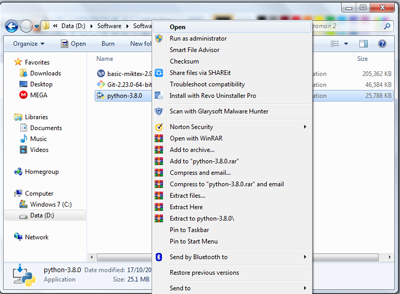
\includegraphics[scale=0.5]{figures/1.png}
    \caption{\textit{install 1}}
    \label{1}
\end{figure}
	
	\item Pilih tempat penyimpanan git, apabila tidak ingin di ubah klik next.

\begin{figure}[H]
    \centering
    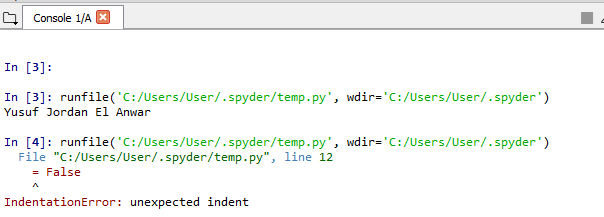
\includegraphics[scale=0.5]{figures/2.png}
    \caption{\textit{install 2}}
    \label{2}
\end{figure}
    
    \item Lalu ada pemilihan komponen, apabila tidak ada yang ingin di tambahkan klik next.

\begin{figure}[H]
    \centering
    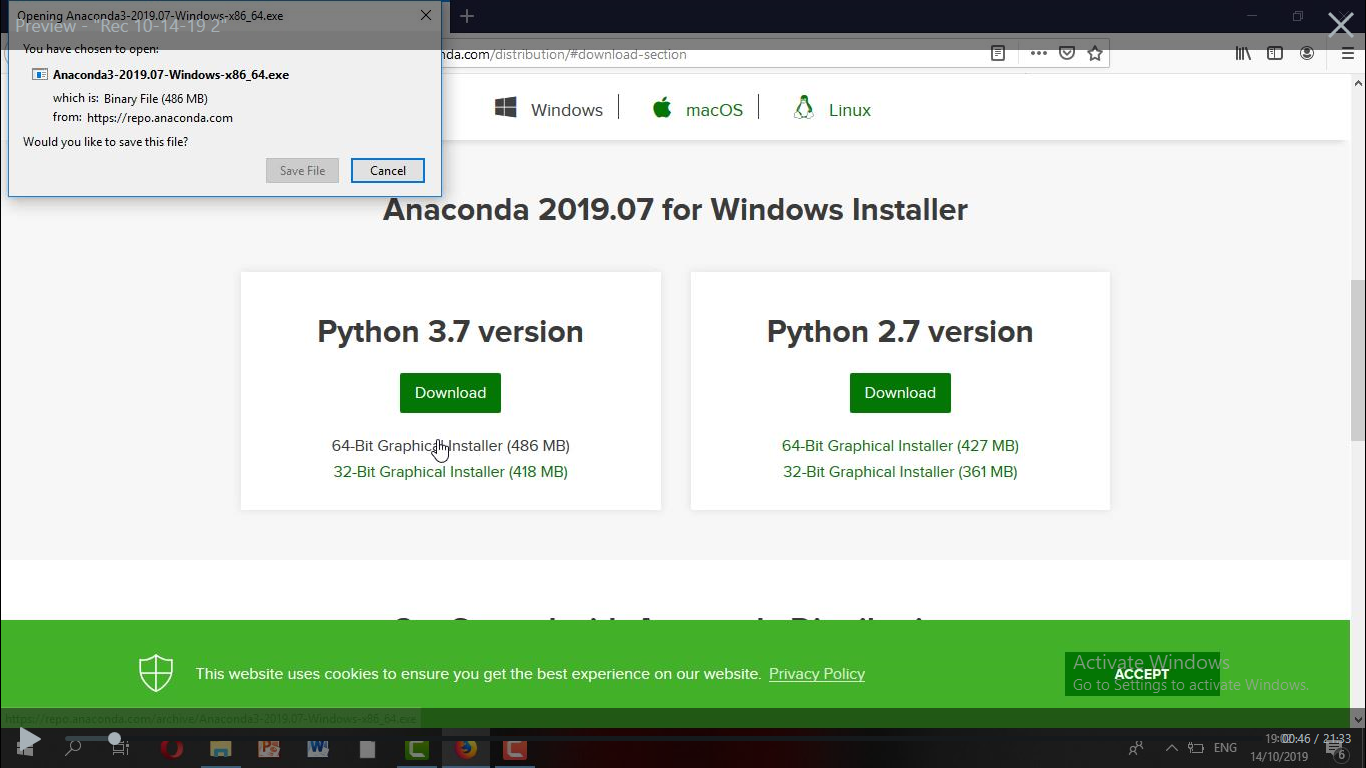
\includegraphics[scale=0.5]{figures/3.png}
    \caption{\textit{install 3}}
    \label{3}
\end{figure}
	
	\item Selanjutnya ada pemilihan direktori start menu, klik next

\begin{figure}[H]
    \centering
    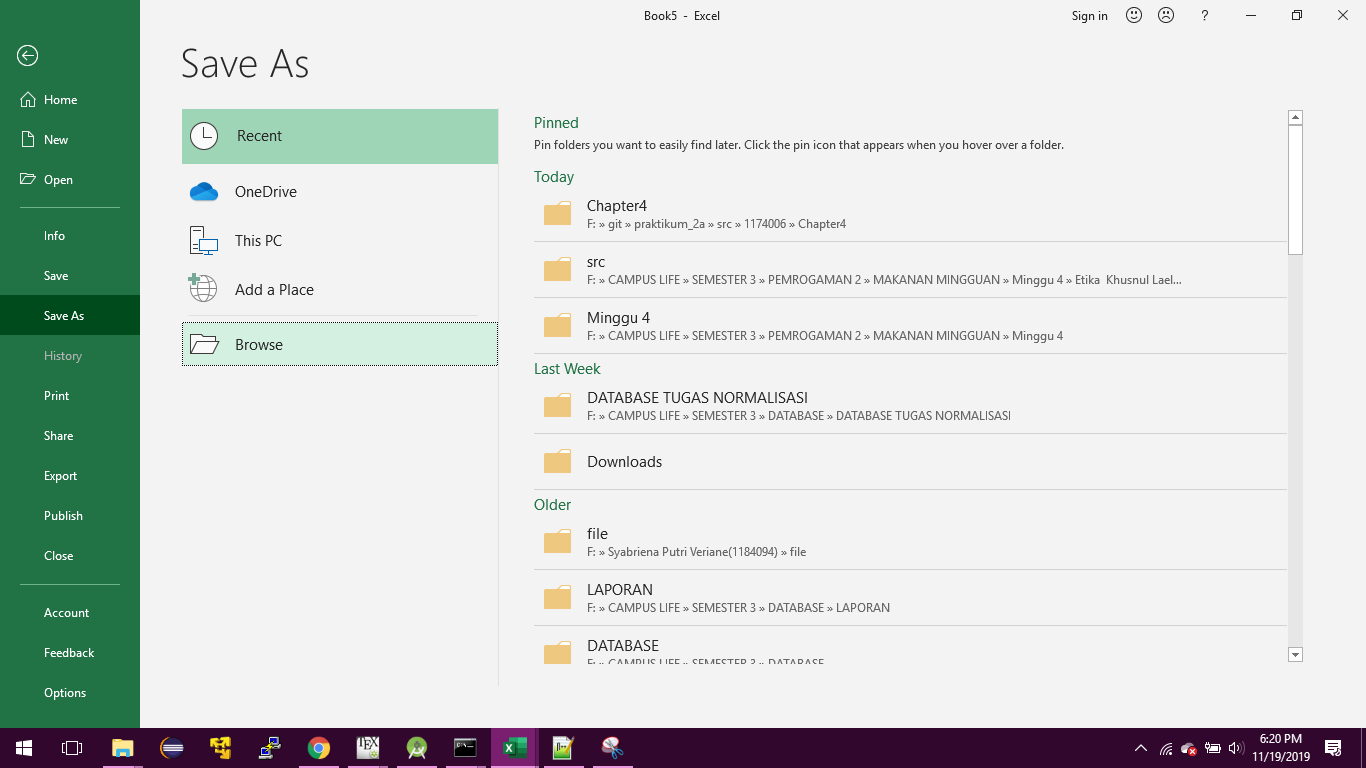
\includegraphics[scale=0.5]{figures/4.png}
    \caption{\textit{install 4}}
    \label{4}
\end{figure}

\end{enumerate}




